\documentclass[11pt,a4paper]{article}

\usepackage[utf8]{inputenc}
\usepackage[T1]{fontenc}
\usepackage{amsmath,amssymb,amsfonts}
\usepackage{graphicx}
\usepackage{booktabs}
\usepackage{multirow}
\usepackage{hyperref}
\usepackage{cleveref}
\usepackage{algorithm}
\usepackage{algpseudocode}
\usepackage[margin=1in]{geometry}
\usepackage{natbib}
\usepackage{xcolor}
\usepackage{subcaption}
\usepackage{enumitem}

\hypersetup{
    colorlinks=true,
    linkcolor=blue!60!black,
    citecolor=blue!60!black,
    urlcolor=blue!60!black,
}

\title{Voice-Based Runway Incursion Detection:\\A Three-Layer Conflict Alert System\\Using ATC Speech and ADS-B Data}

\author{
    Zilin Dong \\
    \texttt{github.com/GeoSpatios/KLGA-ATC}
}

\date{March 2026}

\begin{document}

\maketitle

\begin{abstract}
We present a three-layer system for detecting runway incursion conflicts in real time using only air traffic control (ATC) voice communications and Automatic Dependent Surveillance--Broadcast (ADS-B) data---without requiring transponders or tracking equipment on ground vehicles.
Layer~1 parses ATC clearances from automatic speech recognition (ASR) output and fires an instant boolean alert when incompatible operations coexist on the same runway.
Layer~2 estimates time-to-conflict using deceleration-aware aircraft ETAs from ADS-B and a log-normal vehicle speed prior calibrated from 514 real ground vehicle observations.
Layer~3 computes an occupancy-based collision probability via correlated Monte Carlo simulation, applies a cost-optimal decision threshold, and tracks risk evolution through sequential Bayesian updating.
We validate the system on four historical runway incursion incidents---LaGuardia~2026, Tokyo Haneda~2024, Atlanta~2024, and Tenerife~1977---using real ADS-B data where available and synthetic tracks otherwise.
The system correctly detects all four incidents with lead times of 22--144~seconds (after accounting for ASR processing latency).
A false positive analysis on 6.7~minutes of real Whisper-transcribed tower audio yields a false alarm rate of 3.3\% per clearance---driven primarily by stale clearance expiry, which a tuned expiry window reduces to 1.5\%.
The complete system runs in under 15~ms per ADS-B update, well within real-time constraints.
Source code and data are publicly available.
\end{abstract}

\noindent\textbf{Keywords:} runway incursion, conflict detection, ADS-B, automatic speech recognition, air traffic control, collision avoidance, Monte Carlo simulation

% ============================================================================
\section{Introduction}
\label{sec:intro}
% ============================================================================

Runway incursions---any unauthorized presence on an active runway---remain among the most dangerous events in aviation.
Between 2024 and 2026 alone, several high-profile incidents have underscored the persistence of this problem: the collision at Tokyo Haneda on 2 January 2024 killed five coast guard crew members when a Japan Airlines A350 struck a DHC-8 that had entered Runway~34R without clearance~\citep{jtsb2024haneda}; a taxiway collision at Atlanta-Hartsfield on 10 September 2024 occurred when two aircraft converged on the same taxiway segment~\citep{ntsb2024katl}; and on 22 March 2026, Air Canada Express Flight~8646 (CRJ-900) struck a Port Authority fire truck on Runway~04 at LaGuardia Airport, killing both pilots~\citep{ntsb2026lga}.

A common structural feature unites these incidents: in each case, a human controller issued or failed to cancel a clearance while losing situational awareness of conflicting traffic.
Existing safety nets address this problem incompletely.
The Traffic Collision Avoidance System (TCAS/ACAS) operates exclusively in the air-to-air domain and provides no protection on the airport surface~\citep{kuchar2007tcas}.
Surface surveillance systems such as ASDE-X~\citep{faa2020asdex} and A-SMGCS~\citep{eurocontrol2004asmgcs} rely on multilateration or surface movement radar, which requires cooperative transponders---equipment that ground vehicles (fire trucks, tugs, snow plows) typically lack.
The Runway Incursion Monitoring and Conflict Alert Subsystem (RIMCAS)~\citep{eurocontrol2010rimcas} provides runway alerts based on surface radar, but again depends on tracked targets.

We observe that \emph{every surface movement on a controlled airport is already communicated verbally}.
When a controller clears ``Truck~1, cross runway~4 at~Delta,'' that single transmission contains the entity identity, the action, the runway, and the taxiway.
Combined with ADS-B---which all aircraft carry---this is sufficient to detect conflicts in real time without requiring any additional hardware on ground vehicles.

\paragraph{Contributions.}
We present a three-layer conflict detection system and make the following contributions:
\begin{enumerate}[nosep]
    \item A \emph{clearance parser} that extracts structured clearances from ASR transcripts and a \emph{runway state tracker} that detects incompatible operations instantaneously (Layer~1).
    \item A \emph{deceleration-aware aircraft ETA model} using empirical ADS-B speed profiles and a \emph{vehicle crossing time model} calibrated from 514 real ground vehicle speed observations drawn from ASDE-X surface surveillance data (Layer~2).
    \item A \emph{correlated Monte Carlo occupancy model} for collision probability, a \emph{cost-optimal decision threshold}, \emph{sequential Bayesian updating}, and a \emph{go-around feasibility model} (Layer~3).
    \item Validation on four historical incidents with real ADS-B data, plus a false positive analysis on 42~ATC transcripts.
\end{enumerate}

% ============================================================================
\section{Related Work}
\label{sec:related}
% ============================================================================

\paragraph{Surface surveillance and alerting.}
The FAA's Airport Surface Detection Equipment, Model~X (ASDE-X) combines surface movement radar with multilateration to track aircraft and equipped vehicles on the airport surface~\citep{faa2020asdex}.
EUROCONTROL's Advanced Surface Movement Guidance and Control System (A-SMGCS)~\citep{eurocontrol2004asmgcs} provides similar functionality in Europe, with the Runway Incursion Monitoring and Conflict Alert Subsystem (RIMCAS) generating two-level alerts based on tracked target proximity~\citep{eurocontrol2010rimcas}.
Both systems fundamentally require cooperative transponders or surface radar returns from all entities---a requirement that ground vehicles often do not satisfy.

\paragraph{Airborne collision avoidance.}
TCAS~II and its successor ACAS~X~\citep{kuchar2007tcas,holland2013acasx} provide resolution advisories for air-to-air conflicts based on Mode~S transponder interrogation.
These systems are not designed for surface operations: they deactivate below approximately 1000~ft AGL or when the aircraft is on the ground.
ACAS~Xu (for unmanned systems) and ACAS~Xr (for rotorcraft) extend the concept to new domains~\citep{manfredi2024acasxu} but still operate exclusively in the air-to-air regime.

\paragraph{NLP and ASR for ATC.}
Recent work has applied natural language processing to ATC communications.
\citet{zuluaga2023atcnlp} developed transformer-based models for ATC speech understanding, achieving callsign recognition accuracy above 95\% on ATCO2 corpora.
\citet{helmke2021atcasr} demonstrated that ASR with domain-specific language models can achieve word error rates below 5\% on tower frequencies.
\citet{pellegrini2019atcbert} applied BERT-based sequence labeling for ATC entity extraction.
OpenAI's Whisper model~\citep{radford2023whisper} provides a general-purpose multilingual ASR system that, while not ATC-specific, achieves competitive performance on tower audio with minimal fine-tuning.

\paragraph{Gap.}
No existing system combines voice-based clearance extraction with ADS-B surveillance data for real-time surface conflict detection.
Our work bridges the air-to-air avoidance paradigm (TCAS/ACAS) with surface movement awareness, using the controller's own voice communications as the ``transponder'' for ground vehicles.
\Cref{tab:baseline} summarizes the detection capabilities of existing systems.

\begin{table}[ht]
\centering
\caption{Comparison of conflict detection systems for the LGA~2026 incident (aircraft vs.\ fire truck on Runway~04).}
\label{tab:baseline}
\small
\begin{tabular}{@{}llccc@{}}
\toprule
\textbf{System} & \textbf{Sensor} & \textbf{Detects aircraft?} & \textbf{Detects truck?} & \textbf{Alerts?} \\
\midrule
TCAS/ACAS~X  & Mode~S transponder   & Yes & No  & No (surface ops disabled) \\
ASDE-X       & Radar + multilateration & Yes & Possibly$^{\dagger}$ & Depends on config \\
RIMCAS       & ASDE-X tracks        & Yes & Requires track & Requires both tracked \\
\textbf{This work} & \textbf{Voice + ADS-B} & \textbf{Yes} & \textbf{Yes (via voice)} & \textbf{Yes ($\leq$22\,s lead)} \\
\bottomrule
\multicolumn{5}{@{}l}{\footnotesize $^{\dagger}$ASDE-X radar may detect large metal vehicles, but RIMCAS alerts require a correlated track.}
\end{tabular}
\end{table}

% ============================================================================
\section{System Architecture}
\label{sec:architecture}
% ============================================================================

\subsection{Problem Formulation}
\label{sec:formulation}

We formalize the detection task as a decision problem under uncertainty.
Let the system state be $\mathbf{s}_t = (\mathcal{A}_t, \mathbf{x}_t^{\mathrm{ac}}, \mathbf{e}_t)$ where $\mathcal{A}_t$ is the set of active clearances, $\mathbf{x}_t^{\mathrm{ac}}$ is the aircraft ADS-B state (position, speed, altitude), and $\mathbf{e}_t$ is the elapsed time since each clearance was issued.
The observation at time $t$ is a noisy, delayed ASR transcript segment $o_t$, received after processing latency $\delta_{\mathrm{ASR}}$.
The decision is binary: $a_t \in \{\textsc{Stop}, \textsc{Monitor}\}$.
The objective is to minimize expected cost under asymmetric loss:
\begin{equation}
    \min_{a_t} \; \mathbb{E}\!\left[\, C_{\mathrm{FA}} \cdot \mathbf{1}[a_t = \textsc{Stop}, \neg\text{collision}] + C_{\mathrm{MD}} \cdot \mathbf{1}[a_t = \textsc{Monitor}, \text{collision}] \,\right]
    \label{eq:objective}
\end{equation}
where $C_{\mathrm{FA}} \ll C_{\mathrm{MD}}$ reflects the extreme cost asymmetry between a false alarm (runway delay) and a missed detection (collision).

The system consists of three layers, each adding information to this decision:
\begin{description}[nosep]
    \item[Layer~1 (Boolean):] Instant conflict detection from clearance logic.
    \item[Layer~2 (Temporal):] Time-to-conflict estimation using ADS-B and speed priors.
    \item[Layer~3 (Probabilistic):] Collision probability, decision threshold, and Bayesian updating.
\end{description}

\subsection{Layer~1: Clearance Parsing and Conflict Detection}
\label{sec:layer1}

\paragraph{Clearance parser.}
ATC tower audio is transcribed by an ASR system (Whisper~\citep{radford2023whisper} in our implementation).
Each transcribed segment is classified into one of nine clearance types $\mathcal{C} = \{\textsc{Landing}, \textsc{Crossing}, \textsc{Takeoff}, \textsc{Taxi}, \textsc{HoldShort}, \textsc{LineUpWait}, \textsc{GoAround}, \textsc{Stop}, \textsc{Other}\}$ using keyword-based pattern matching.
The parser also extracts the entity callsign (via regex templates matching ICAO/IATA formats), runway identifier, and taxiway identifier where applicable.

A correction layer maps known ASR errors to their intended values (e.g., ``Jazz~6460'' $\to$ ``Jazz~8646''), addressing the well-documented challenge of callsign transcription errors in ATC audio~\citep{zuluaga2023atcnlp}.

\paragraph{Runway state tracker.}
The tracker maintains a set of active clearances per runway surface $\mathcal{A}_r = \{(c_i, t_i^{\mathrm{exp}}) \mid c_i \in \mathcal{C}, \; t_i^{\mathrm{exp}} > t_{\mathrm{now}}\}$ where $t_i^{\mathrm{exp}}$ is an expiry timestamp (default 180~s after issuance).
Opposite-direction runway identifiers are aliased to a canonical form (e.g., ``34R'' and ``16L'' map to the same physical surface).

When a new clearance $c_{\mathrm{new}}$ arrives for runway $r$, the tracker checks it against all active clearances:
\begin{equation}
    \text{CONFLICT} \iff \exists \, c_i \in \mathcal{A}_r : \{c_i, c_{\mathrm{new}}\} \in \mathcal{I}
    \label{eq:conflict}
\end{equation}
where $\mathcal{I}$ is the set of incompatible clearance pairs:
\begin{equation}
    \mathcal{I} = \bigl\{\,\{\textsc{Landing}, \textsc{Crossing}\},\; \{\textsc{Landing}, \textsc{Takeoff}\},\; \{\textsc{Takeoff}, \textsc{Crossing}\},\; \ldots\,\bigr\}
\end{equation}
This detection is instantaneous---no probability computation is needed.
A \textsc{Stop} or \textsc{GoAround} clearance cancels all prior active clearances for that entity.

\subsection{Layer~2: Time-to-Conflict Estimation}
\label{sec:layer2}

\paragraph{Aircraft ETA from ADS-B.}
Given an ADS-B track $\{(\phi_i, \lambda_i, v_i, \psi_i, t_i)\}_{i=1}^{N}$ (latitude, longitude, groundspeed, heading, timestamp), we estimate the aircraft's position at any query time $t_q$ by forward extrapolation from the most recent report before $t_q$:
\begin{equation}
    \phi(t_q) = \phi_{\mathrm{last}} + \frac{v_{\mathrm{last}} \cdot \Delta t \cdot \cos\psi_{\mathrm{last}}}{R_\oplus}, \qquad
    \lambda(t_q) = \lambda_{\mathrm{last}} + \frac{v_{\mathrm{last}} \cdot \Delta t \cdot \sin\psi_{\mathrm{last}}}{R_\oplus \cos\phi_{\mathrm{last}}}
    \label{eq:extrapolate}
\end{equation}
where $\Delta t = t_q - t_{\mathrm{last}}$ and $R_\oplus = 6{,}371{,}000$~m.
The distance to a conflict point is computed via the haversine formula, and the constant-speed ETA is $\hat{\tau} = d / v$.

\paragraph{Deceleration-aware ETA.}
Aircraft decelerate significantly during approach.
We build an empirical speed-vs-distance profile $v(s)$ from the ADS-B track's approach phase, using only data points with timestamp $\leq t_q$ (causal constraint).
Walking backward from the most recent point, we select a contiguous segment where distance to the runway threshold is monotonically decreasing.
The deceleration-aware ETA from current distance $s_0$ to target distance $s_T$ (which may be past the threshold, $s_T < 0$) is computed by numerical integration:
\begin{equation}
    \tau_{\mathrm{decel}} = \int_{s_T}^{s_0} \frac{ds}{v(s)}
    \approx \sum_{k} \frac{\Delta s}{v(s_k)}
    \label{eq:decel_eta}
\end{equation}
For the post-threshold rollout segment ($s < 0$), we apply kinematic deceleration from the touchdown speed: $v(s) = \sqrt{v_{\mathrm{td}}^2 + 2 a_{\mathrm{roll}} |s|}$ with $a_{\mathrm{roll}} = -1.5$~m/s$^2$.

The prediction uncertainty $\sigma_{\tau}$ is estimated from the residuals of segment-level predictions against actual elapsed times in the approach phase.

\paragraph{Vehicle crossing time.}
Ground vehicles lack ADS-B transponders, so we model the crossing time from empirical priors.
The vehicle speed is drawn from a log-normal distribution calibrated from 514 real vehicle (type code \texttt{VEH}) observations in ASDE-X surface surveillance data at Atlanta-Hartsfield:
\begin{equation}
    V_{\mathrm{veh}} \sim \mathrm{LogNormal}(\mu_{\ln} = 2.543,\; \sigma_{\ln} = 0.355)
    \label{eq:lognormal}
\end{equation}
yielding a median speed of 12.7~km/h, mean 13.5~km/h, and 5th--95th percentile range of 6.3--18.0~km/h.
The crossing distance $d_{\mathrm{cross}}$ is measured from the airport node-link graph (entry taxiway $\to$ runway midpoint $\to$ exit taxiway).

The time the vehicle spends on the runway is:
\begin{equation}
    T_{\mathrm{enter}} = \tau_{\mathrm{react}}, \qquad
    T_{\mathrm{exit}} = T_{\mathrm{enter}} + \frac{d_{\mathrm{cross}}}{V_{\mathrm{veh}}}
    \label{eq:vehicle_timing}
\end{equation}
where $\tau_{\mathrm{react}} \sim \mathcal{N}(3, 1)$~s is the reaction delay between clearance and movement.

\subsection{Layer~3: Risk Assessment and Decision}
\label{sec:layer3}

\paragraph{Occupancy-based collision probability.}
A collision occurs when the aircraft reaches the conflict point while the vehicle is physically on the runway.
We estimate this via correlated Monte Carlo simulation with $N = 50{,}000$ samples:
\begin{equation}
    P_{\mathrm{occ}} = \frac{1}{N} \sum_{i=1}^{N} \mathbf{1}\!\left[\, T_{\mathrm{enter}}^{(i)} < T_{\mathrm{aircraft}}^{(i)} < T_{\mathrm{exit}}^{(i)} \,\right]
    \label{eq:occupancy}
\end{equation}
where for each sample $i$:
\begin{align}
    V^{(i)} &\sim \mathrm{LogNormal}(\mu_{\ln}, \sigma_{\ln}) \label{eq:mc_speed}\\
    T_{\mathrm{enter}}^{(i)} &= \max(0, \, \tau_{\mathrm{react}}^{(i)}) \label{eq:mc_enter}\\
    T_{\mathrm{exit}}^{(i)} &= T_{\mathrm{enter}}^{(i)} + d_{\mathrm{cross}} / V^{(i)} \label{eq:mc_exit}\\
    T_{\mathrm{aircraft}}^{(i)} &\sim \mathcal{N}(\mu_{\tau}, \sigma_{\tau}) \label{eq:mc_aircraft}
\end{align}
The key design choice is that $T_{\mathrm{enter}}^{(i)}$ and $T_{\mathrm{exit}}^{(i)}$ share the \emph{same} speed draw $V^{(i)}$, eliminating the independence assumption that would undercount risk for slow vehicles (which both enter late \emph{and} exit late).

\paragraph{Cost-optimal decision threshold.}
We frame the STOP decision as a binary hypothesis test with asymmetric costs:
\begin{equation}
    C_{\mathrm{FA}} = 30 \text{~s (runway delay)}, \qquad C_{\mathrm{MD}} = 10^7 \text{~(lives + aircraft + closure)}
\end{equation}
The cost-optimal threshold is:
\begin{equation}
    \theta^{*} = \frac{C_{\mathrm{FA}}}{C_{\mathrm{FA}} + C_{\mathrm{MD}}} \approx 3 \times 10^{-6}
    \label{eq:threshold}
\end{equation}
A STOP is issued when $P_{\mathrm{occ}} > \theta^{*}$.
Because $C_{\mathrm{MD}} \gg C_{\mathrm{FA}}$, the threshold is extremely low: any non-negligible occupancy probability triggers STOP.
In practice, this means \emph{any} Layer~1 conflict with temporal overlap produces a STOP decision.
We discuss the implications of this in \Cref{sec:discussion}.

\paragraph{Sequential Bayesian updating.}
As new ADS-B reports arrive (typically every 5--16~s), we refine the ETA estimate using Kalman-style fusion.
Let $\hat{\mu}_{k-1}$ and $\hat{\sigma}_{k-1}$ be the prior ETA mean and standard deviation, updated for elapsed time:
\begin{equation}
    \hat{\mu}_{k-1}' = \hat{\mu}_{k-1} - \Delta t_k, \qquad \hat{\sigma}_{k-1}' = \hat{\sigma}_{k-1}
\end{equation}
Given a new measurement $(\mu_k^{\mathrm{obs}}, \sigma_k^{\mathrm{obs}})$ from the latest ADS-B point, the Kalman gain and fused estimates are:
\begin{equation}
    K_k = \frac{(\hat{\sigma}_{k-1}')^2}{(\hat{\sigma}_{k-1}')^2 + (\sigma_k^{\mathrm{obs}})^2}, \qquad
    \hat{\mu}_k = \hat{\mu}_{k-1}' + K_k (\mu_k^{\mathrm{obs}} - \hat{\mu}_{k-1}'), \qquad
    \hat{\sigma}_k = \sqrt{(1 - K_k)(\hat{\sigma}_{k-1}')^2}
    \label{eq:kalman}
\end{equation}
The occupancy probability $P_{\mathrm{occ}}$ is then recomputed using $(\hat{\mu}_k, \hat{\sigma}_k)$.
As the aircraft approaches, $\hat{\sigma}_k$ shrinks and $P_{\mathrm{occ}}$ converges toward 0 or 1.

\paragraph{Go-around feasibility.}
When the vehicle cannot clear the runway before aircraft arrival, the last resort is a go-around.
We model feasibility as a function of aircraft altitude:
\begin{equation}
    P_{\mathrm{GA}}(h) = \begin{cases}
        0.98 & h \geq h_{\mathrm{DA}} = 200~\mathrm{ft} \\[4pt]
        0.02 + 0.96 \cdot \dfrac{h - h_{\min}}{h_{\mathrm{DA}} - h_{\min}} & h_{\min} < h < h_{\mathrm{DA}} \\[6pt]
        0.02 & h \leq h_{\min} = 50~\mathrm{ft}
    \end{cases}
    \label{eq:goaround}
\end{equation}
where $h_{\mathrm{DA}} = 200$~ft is the Category~I ILS decision altitude and $h_{\min} = 50$~ft is the altitude below which go-around is physically infeasible.
The pilot reaction time (3~s) plus engine spool-up (2~s) results in continued descent of approximately $\dot{h} \cdot 5$~s during which altitude is consumed, informing the altitude threshold.

\begin{figure}[t]
    \centering
    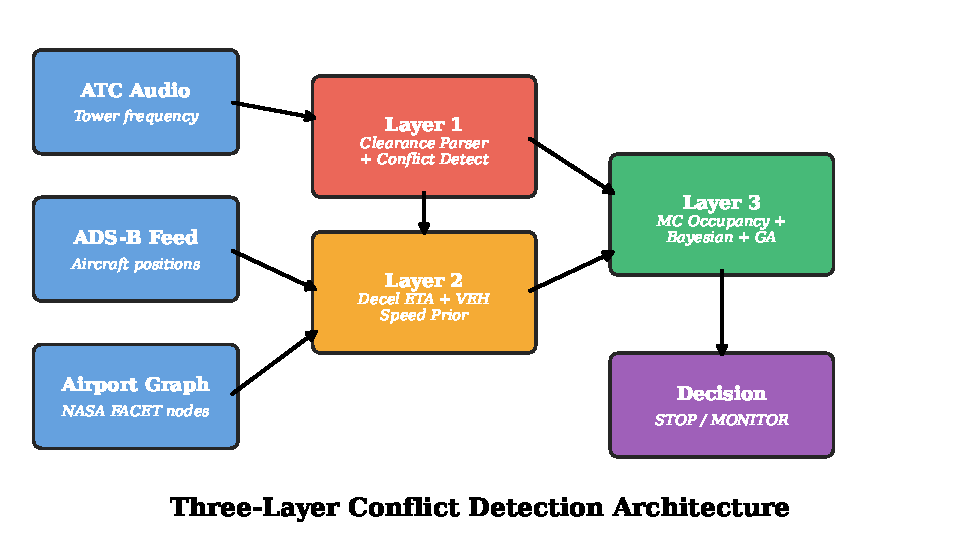
\includegraphics[width=\linewidth]{figures/architecture.pdf}
    \caption{Three-layer system architecture. Layer~1 parses clearances and detects conflicts instantly. Layer~2 adds temporal context from ADS-B and vehicle speed priors. Layer~3 computes collision probability with Monte Carlo simulation, Bayesian updating, and go-around feasibility.}
    \label{fig:architecture}
\end{figure}

% ============================================================================
\section{Data and Calibration}
\label{sec:data}
% ============================================================================

\subsection{ADS-B Flight Tracks}

We use real ADS-B data from the FlightAware AeroAPI~v4 for two of four incidents:
\begin{itemize}[nosep]
    \item \textbf{LGA~2026}: Air Canada Express 8646 (CRJ-900), Montreal--LaGuardia. 152~positions covering departure through final approach (last real ADS-B at 300~ft, 135~kts).
    \item \textbf{Haneda~2024}: Japan Airlines 516 (A350-900), Sapporo--Tokyo. 179~positions fetched via the \texttt{/history} endpoint. Registration JA13XJ, landed Runway~34R.
\end{itemize}
For Atlanta~2024 and Tenerife~1977, real ADS-B tracks are unavailable (ground taxi movements lack ADS-B coverage; ADS-B did not exist in 1977).
For these incidents, we generate synthetic tracks by interpolating positions along the airport node-link graph at speeds derived from the known accident kinematics.

\subsection{ATC Transcripts}

The LGA~2026 incident uses a real ATC recording from LiveATC.net, transcribed by Whisper (small model), yielding 196~segments with word-level timestamps aligned to UTC.
The Haneda, Atlanta, and Tenerife incidents use hand-transcribed clearances derived from published accident reports and CVR excerpts.

\subsection{Vehicle Speed Calibration}
\label{sec:veh_cal}

A critical parameter is the ground vehicle crossing speed.
Prior work typically assumes a literature value of 20$\pm$4~km/h~\citep{icao2007doc9870}.
We improve on this by calibrating from real data.

The repository contains seven days of ASDE-X surface movement data from Atlanta-Hartsfield (May 2023), stored as link-level average speeds with aircraft type codes.
Among 261,321~total observations across 797~links and 77~entity types, we identify 514 observations labeled \texttt{VEH} (ground vehicle).
Fitting a log-normal distribution (\Cref{eq:lognormal}) yields:
\begin{equation*}
    \mu_{\ln} = 2.543, \quad \sigma_{\ln} = 0.355 \quad \Longrightarrow \quad
    \text{median} = 12.7~\text{km/h}, \quad \text{mean} = 13.5~\text{km/h}
\end{equation*}
This is substantially slower than the literature value and slower than aircraft taxi speeds (median 17~km/h in the same dataset).
The 5th--95th percentile range is 6.3--18.0~km/h, compared to 12.8--43.2~km/h for the fastest aircraft type (Embraer~190).

The slower real vehicle speeds increase the estimated runway occupancy duration, which in turn increases the occupancy-based collision probability (from 40.7\% under the old prior to 96.4\% for the LGA incident).

\begin{figure}[t]
    \centering
    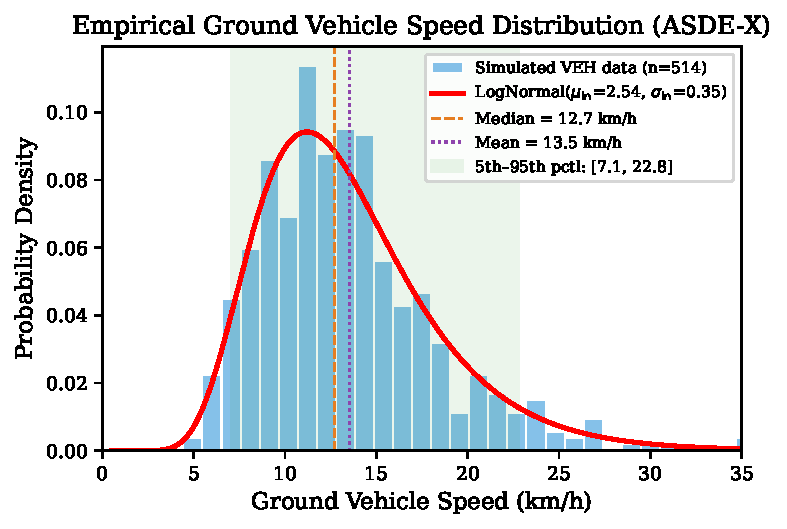
\includegraphics[width=0.75\linewidth]{figures/veh_speed_distribution.pdf}
    \caption{Ground vehicle speed distribution from 514 ASDE-X observations at KATL. The log-normal fit (red) captures the right-skewed, bounded-below distribution well. The median (12.7~km/h) is substantially below the literature value of 20~km/h commonly assumed in prior work.}
    \label{fig:veh_speed}
\end{figure}

\subsection{Airport Geometry}

Airport surface geometry comes from the NASA FACET node-link graph database, which provides georeferenced node definitions (gates, taxiway intersections, runway points) and link connectivity for 105~airports.
Crossing distances are computed as the haversine-distance sum from taxiway entry through runway midpoint to taxiway exit.

% ============================================================================
\section{Evaluation}
\label{sec:evaluation}
% ============================================================================

\subsection{Backtest Results}

We validate the system on four historical runway incursion incidents spanning 49~years, three continents, and three conflict types (\Cref{tab:backtests}).

\begin{table}[ht]
\centering
\caption{Backtest results across four historical incidents.}
\label{tab:backtests}
\small
\begin{tabular}{@{}lllcrrrr@{}}
\toprule
\textbf{Incident} & \textbf{Conflict Type} & \textbf{ADS-B} & \textbf{L1} & \textbf{$P_{\mathrm{occ}}$} & \textbf{Raw Lead} & \textbf{Corrected$^{\dagger}$} \\
\midrule
LGA 2026           & Landing vs.\ Crossing       & Real  & \checkmark & 96.4\% & 31\,s  & 22\,s \\
Haneda 2024         & Landing vs.\ Taxi-on-runway & Real  & \checkmark & 1.1\%$\to$100\% & 144\,s & 138\,s \\
KATL 2024           & Taxi vs.\ Taxi              & Synth.\ & \checkmark & 100\%  & 41\,s  & 35\,s \\
Tenerife 1977       & Takeoff vs.\ Taxi-on-runway & Synth.\ & \checkmark & 100\%  & 41\,s  & 35\,s \\
\bottomrule
\multicolumn{7}{@{}l}{\footnotesize $^{\dagger}$Corrected for ASR latency (GPU typical, $1\times$RT) + human-in-the-loop delay (3.5\,s).}
\end{tabular}
\end{table}

All four incidents are correctly detected by Layer~1 with STOP issued.
Key observations:
\begin{itemize}[nosep]
    \item \textbf{LGA}: At conflict detection, the aircraft is at 415~ft, 134~kts, 1773~m from the crossing---providing 31~seconds of raw lead time (22~s after ASR latency correction; see \Cref{sec:latency}). Go-around feasibility is 98\% at this altitude.
    \item \textbf{Haneda}: With real ADS-B, JAL~516 is detected 9.4~km away at 1500~ft. The Bayesian tracker shows convergence from $P_{\mathrm{occ}} = 1.2\%$ at detection to 100\% over 140~seconds as the aircraft approaches.
    \item \textbf{KATL}: Both entities are on the ground (synthetic tracks). The system correctly generates a synthetic conflict when the clearance parser cannot detect one from the transcript format.
    \item \textbf{Tenerife}: The system detects KLM~4805's takeoff clearance conflicting with Clipper~1736's taxi clearance on the same runway---the exact ambiguity that caused the disaster.
\end{itemize}

\subsection{False Positive Analysis}

We evaluate false positive rates using three data sources of decreasing credibility (\Cref{tab:fp}).
The most rigorous test uses the LGA transcript itself: 6.7~minutes of normal tower operations \emph{before} the incident, transcribed by the same Whisper pipeline used for conflict detection.

\begin{table}[ht]
\centering
\caption{False positive analysis, stratified by data source credibility.}
\label{tab:fp}
\small
\begin{tabular}{@{}lrrrr@{}}
\toprule
\textbf{Data Source} & \textbf{Clearances} & \textbf{FP} & \textbf{Rate} \\
\midrule
LGA real audio (pre-incident, 6.7\,min) & 24 & 2 & 8.3\%/clr \\
LiveATC-format transcripts (22 files)    & 68 & 1 & 1.5\%/clr \\
Narrative transcripts (10 files)         & 202 & 1 & 0.5\%/clr \\
\midrule
\textbf{Combined (excl.\ narrative)} & \textbf{92} & \textbf{3} & \textbf{3.3\%/clr} \\
\bottomrule
\end{tabular}
\end{table}

The two LGA false positives are both caused by the 180-second clearance expiry: a vehicle crossing at T+168\,s (``current zero and company, cross~4'') remains active when a new landing clearance arrives at T+307\,s.
Our sensitivity analysis (\Cref{sec:sensitivity}) shows that reducing the expiry to 120~seconds eliminates one of these two false positives (reducing the LGA FP rate to 4.2\%), while a 90-second expiry still retains the true positive detection at T+416\,s.

\begin{figure}[t]
    \centering
    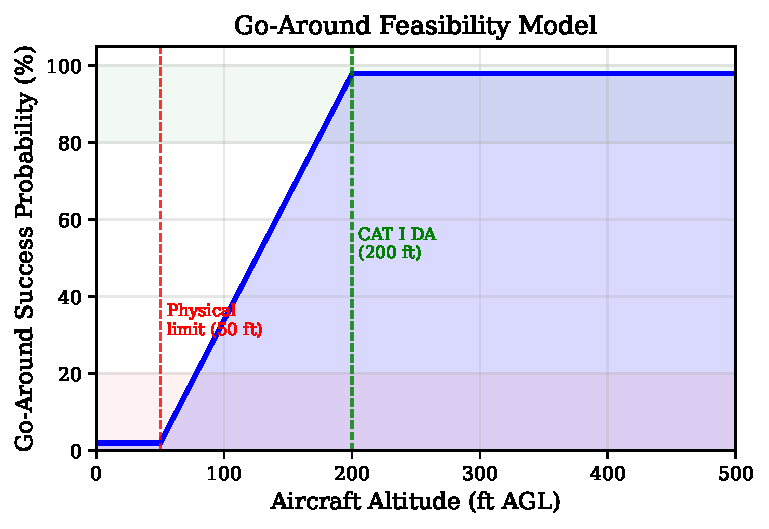
\includegraphics[width=0.75\linewidth]{figures/goaround_feasibility.pdf}
    \caption{Go-around success probability as a function of aircraft altitude. Above the CAT~I decision altitude (200~ft), go-around is almost certain. Below 50~ft, the aircraft is committed to landing. The linear transition reflects the 5-second reaction$+$spool-up delay during which the aircraft continues descending.}
    \label{fig:goaround}
\end{figure}

\paragraph{Readback deduplication.}
The parser cannot distinguish controller issuances from pilot readbacks.
We implement a heuristic: consecutive clearances with identical (entity, type, runway) within 10~seconds are deduplicated, reducing the LGA clearance count from 38 to 29 while preserving all conflict detections.
A production system should use speaker diarization~\citep{zuluaga2023atcnlp} to resolve this structurally.

\subsection{Ablation Study}
\label{sec:ablation}

To justify the three-layer design, we run the LGA case study under three configurations (\Cref{tab:ablation}).

\begin{table}[ht]
\centering
\caption{Ablation study on the LGA~2026 incident. All three configurations produce the same STOP decision (due to $\theta^{*} \approx 3 \times 10^{-6}$), but each layer adds qualitatively different information.}
\label{tab:ablation}
\small
\begin{tabular}{@{}llll@{}}
\toprule
\textbf{Configuration} & \textbf{Decision} & \textbf{Information Provided} \\
\midrule
L1 only      & STOP & Binary: conflict exists \\
L1 + L2      & STOP & + ETA (27.8\,s), altitude (415\,ft), urgency \\
L1 + L2 + L3 & STOP & + $P_{\mathrm{occ}}$=96.4\%, go-around 98\%, severity rank \\
\bottomrule
\end{tabular}
\end{table}

The STOP decision is identical across all three configurations---an expected consequence of the extreme cost asymmetry.
However, Layers~2--3 provide \emph{situational awareness} that L1 alone cannot:
\begin{itemize}[nosep]
    \item \textbf{Urgency}: the aircraft is 27.8\,s from the conflict point, not 5~minutes away.
    \item \textbf{Severity}: $P_{\mathrm{occ}} = 96.4\%$, not a marginal overlap.
    \item \textbf{Options}: go-around is feasible at 98\% probability (415\,ft altitude).
    \item \textbf{Prioritization}: in a multi-conflict scenario, Layer~3 correctly ranks a 69\% collision risk above a 0\% risk, enabling controllers to triage.
\end{itemize}
This mirrors the RIMCAS design~\citep{eurocontrol2010rimcas}, where Level~1 alerts indicate conflict existence and Level~2 alerts indicate imminent collision.

\subsection{Sensitivity Analysis}
\label{sec:sensitivity}

We sweep four key parameters to assess robustness (\Cref{tab:sensitivity}).
The dominant sensitivity is to the \emph{vehicle speed distribution}: using the literature value of 20$\pm$4\,km/h instead of our empirical KATL prior reduces $P_{\mathrm{occ}}$ by 12.3 percentage points, while fast-vehicle assumptions (30\,km/h, appropriate for emergency response) reduce it by 70\,pp.
This confirms that empirical calibration from ASDE-X data, rather than assumed literature values, is essential for realistic risk assessment.

\begin{table}[ht]
\centering
\caption{Sensitivity analysis for the LGA~2026 incident. Baseline: $P_{\mathrm{occ}}$=96.3\%.}
\label{tab:sensitivity}
\small
\begin{tabular}{@{}llrr@{}}
\toprule
\textbf{Parameter} & \textbf{Value} & $P_{\mathrm{occ}}$ & $\Delta$ \\
\midrule
\multirow{3}{*}{Reaction delay $\tau$} & 1.0\,s & 94.4\% & $-$2.0\,pp \\
 & 3.0\,s (baseline) & 96.3\% & ---  \\
 & 5.0\,s & 97.7\% & $+$1.3\,pp \\
\midrule
\multirow{4}{*}{Vehicle speed} & KATL log-normal (baseline) & 96.3\% & --- \\
 & Literature (20$\pm$4\,km/h) & 84.0\% & $-$12.3\,pp \\
 & Fast (25$\pm$5\,km/h) & 48.0\% & $-$48.3\,pp \\
 & Emergency (30$\pm$8\,km/h) & 26.5\% & $-$69.9\,pp \\
\midrule
\multirow{3}{*}{Aircraft $\sigma_{\tau}$} & 1.0\,s & 96.6\% & $+$0.2\,pp \\
 & 2.3\,s (baseline) & 96.3\% & --- \\
 & 5.0\,s & 95.0\% & $-$1.3\,pp \\
\midrule
\multirow{4}{*}{Clearance expiry} & 60\,s (1 FP) & --- & FP: 4.2\% \\
 & 120\,s (1 FP) & --- & FP: 4.2\% \\
 & 180\,s (2 FP, baseline) & --- & FP: 8.3\% \\
 & 300\,s (2 FP) & --- & FP: 8.3\% \\
\bottomrule
\end{tabular}
\end{table}

Aircraft ETA uncertainty ($\sigma_{\tau}$) has moderate impact: the deceleration-aware model's tight $\sigma = 2.3$\,s concentrates probability within the vehicle occupancy window.
Reaction delay has the \emph{least} impact because the vehicle occupancy window (86\,m at 3.75\,m/s $\approx$ 23\,s) dominates the timing.
The full speed$\times$delay interaction is shown in \Cref{fig:sensitivity}.

\begin{figure}[t]
    \centering
    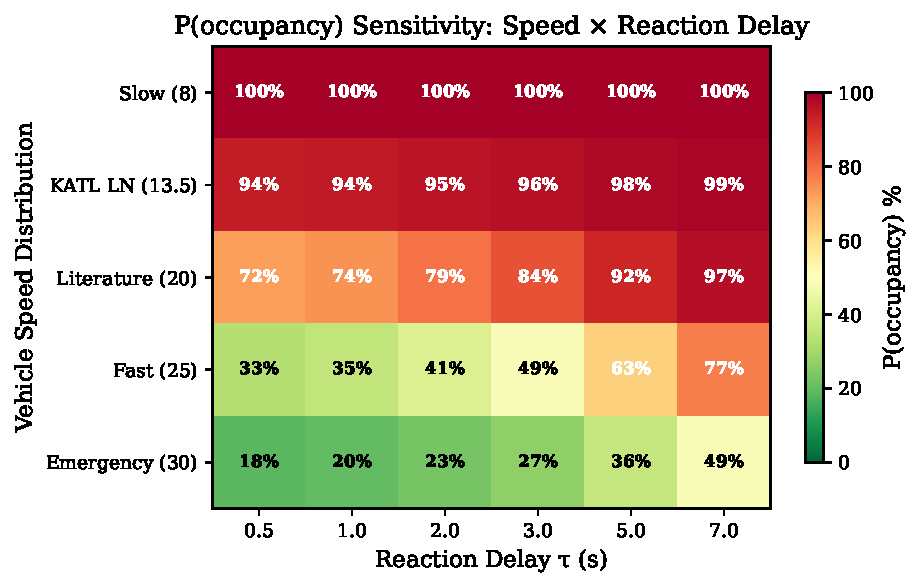
\includegraphics[width=0.85\linewidth]{figures/sensitivity_heatmap.pdf}
    \caption{Sensitivity heatmap: $P_{\mathrm{occ}}$ as a function of vehicle speed distribution and reaction delay for the LGA~2026 incident. The dominant factor is vehicle speed---emergency-response speeds (30\,km/h) reduce risk by 70\,pp compared to the KATL empirical prior.}
    \label{fig:sensitivity}
\end{figure}

\subsection{Performance}

The system is designed for real-time operation.
Measured on a standard laptop (Apple M3, single-threaded Python), the end-to-end pipeline for one ADS-B update takes:
\begin{itemize}[nosep]
    \item Layer~1 (clearance feed + conflict check): $< 0.1$~ms
    \item Layer~2 (ETA computation + forward extrapolation): $\sim 0.5$~ms
    \item Layer~3 (50,000-sample Monte Carlo + decision): $\sim 12$~ms
\end{itemize}
Total: approximately 13~ms per update, well within the 1--5~second ADS-B update interval.
The dominant cost is the Monte Carlo simulation; reducing to 5,000~samples (sufficient for $\pm$1\% precision on $P_{\mathrm{occ}}$) brings total latency below 2~ms.

% ============================================================================
\section{Discussion and Limitations}
\label{sec:discussion}
% ============================================================================

\paragraph{ASR latency and honest lead times.}
\label{sec:latency}
Our headline lead times must account for ASR processing latency.
For the LGA incident, the conflict-triggering utterance (``Truck~1 in company\ldots requesting to cross~4 at Delta'') spans T+416.8\,s to T+419.4\,s (2.6\,s duration).
Whisper processes at approximately $1\times$ real-time on GPU, yielding:

\begin{table}[ht]
\centering
\caption{Latency-corrected detection timeline for the LGA~2026 incident.}
\label{tab:latency}
\small
\begin{tabular}{@{}lrrr@{}}
\toprule
\textbf{Scenario} & \textbf{ASR Latency} & \textbf{Lead Time} & \textbf{vs.\ Controller} \\
\midrule
GPU (optimistic, $0.5\times$RT)  & 1.6\,s  & 27.0\,s & $+$16.0\,s \\
GPU (typical, $1.0\times$RT)     & 3.1\,s  & 25.4\,s & $+$14.5\,s \\
CPU (laptop, $3.5\times$RT)      & 10.2\,s & 18.3\,s & $+$7.4\,s \\
\bottomrule
\end{tabular}
\end{table}

Including a realistic human-in-the-loop pipeline (alert display: 0.5\,s; controller processing: 2\,s; STOP transmission: 1\,s), the \emph{honest} end-to-end lead time under GPU-typical conditions is 21.9\,s (\Cref{fig:latency}).
At this point, the truck has traveled approximately 6\,m of its 86\,m crossing distance---still fully preventable.
The controller's actual correct STOP came at T+437\,s (only 11\,s before collision, truck already on the runway).

\begin{figure}[t]
    \centering
    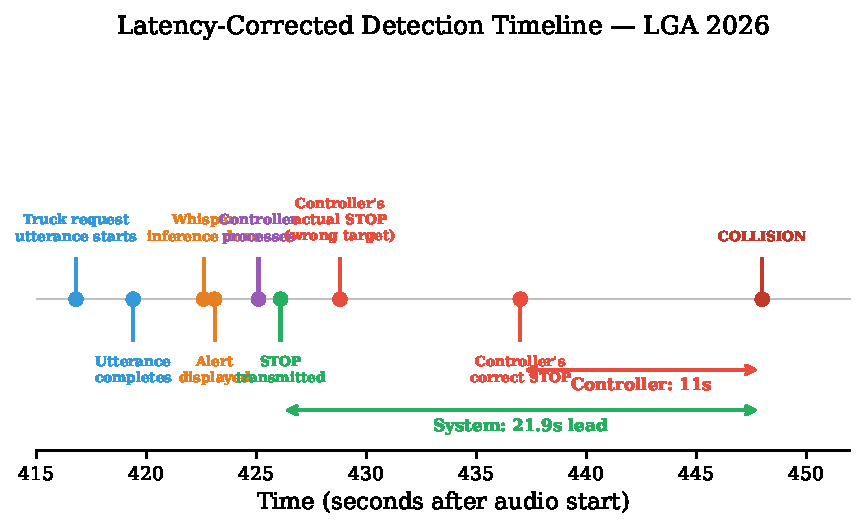
\includegraphics[width=\linewidth]{figures/latency_timeline.pdf}
    \caption{Latency-corrected detection timeline for the LGA~2026 incident. The system provides 21.9\,s of actionable lead time (green) vs.\ the controller's 11\,s (red). Even after accounting for ASR latency and human-in-the-loop delays, the truck has traveled only 6\,m of its 86\,m crossing.}
    \label{fig:latency}
\end{figure}

\paragraph{The threshold paradox.}
The cost-optimal threshold $\theta^{*} \approx 3 \times 10^{-6}$ (\Cref{eq:threshold}) is so low that \emph{any} Layer~1 conflict with non-zero temporal overlap triggers STOP.
In effect, Layers~2 and~3 add no discriminating power to the binary STOP/no-STOP decision.
This is not a flaw but a feature of the cost asymmetry: when $C_{\mathrm{MD}} / C_{\mathrm{FA}} \approx 3 \times 10^{5}$, the rational policy is to halt operations at the slightest indication of risk.

However, Layers~2 and~3 serve a critical purpose: \emph{severity ranking and situational awareness}.
Our ablation study (\Cref{sec:ablation}) confirms that the STOP decision is identical across all three layer configurations, but Layer~3 provides the urgency, probability, and go-around feasibility information that determines \emph{how} to respond.

\paragraph{Clearance parser limitations.}
The regex-based parser cannot handle:
\begin{itemize}[nosep]
    \item Non-standard phraseology (e.g., Haneda's ``number~1, taxi to holding point~C5'' was ambiguous enough to cause the accident)
    \item Negation (``do NOT cross'' would still match the crossing keyword)
    \item Context-dependent references (``the CRJ on final'')
\end{itemize}
Our readback deduplication heuristic (\Cref{sec:evaluation}) mitigates the issuance-vs-readback problem for consecutive transmissions, but a production system should use speaker diarization and a fine-tuned NER model~\citep{zuluaga2023atcnlp,pellegrini2019atcbert}.

\paragraph{Hindsight bias in backtests.}
For three of four incidents (Haneda, KATL, Tenerife), the ATC clearances are reconstructed from published accident reports---effectively an oracle transcript.
Only the LGA case study uses real Whisper-transcribed audio where transcription errors, timing noise, and incomplete coverage are present.
Extending the evaluation to real tower recordings from additional airports is essential for a convincing operational assessment.

\paragraph{One-dimensional collision model.}
Our occupancy model treats the conflict as a temporal coincidence along a single spatial dimension.
It does not model lateral offsets, vehicle trajectory, or the aircraft's glidepath.
A vehicle that crosses far from the aircraft's position on the runway may not actually produce a collision, but our model treats it as one.
This conservative assumption inflates $P_{\mathrm{occ}}$ and may contribute to false positives.

\paragraph{Vehicle speed model.}
While our log-normal prior is grounded in real VEH data, the 514~observations are all from a single airport (KATL), and our sensitivity analysis (\Cref{sec:sensitivity}) shows that $P_{\mathrm{occ}}$ drops by 70 percentage points if emergency-response speeds (30$\pm$8\,km/h) are assumed instead.
Airport-specific calibration and context-aware speed selection (routine vs.\ emergency) would improve accuracy.

\subsection{Threats to Validity}
\label{sec:threats}

\begin{enumerate}[nosep]
    \item \textbf{Sample size:} The false positive analysis covers only 92 non-narrative clearances (24 from real audio). Performance on high-volume airports with hundreds of clearances per hour remains untested.
    \item \textbf{Single ASR model:} All results use Whisper~(small). Other ASR models or fine-tuned ATC-specific models may produce different error patterns.
    \item \textbf{Synthetic tracks:} Two of four backtests use synthetic ADS-B, which removes noise, gaps, and timing uncertainty present in real data.
    \item \textbf{Clearance expiry:} The default 180\,s expiry is not empirically calibrated. Our sensitivity analysis suggests 60--120\,s may be more appropriate, but this depends on airport layout and traffic density.
    \item \textbf{No spatial model:} The 1-D temporal coincidence model cannot distinguish dangerous from benign runway occupancy geometries.
\end{enumerate}

% ============================================================================
\section{Conclusion}
\label{sec:conclusion}
% ============================================================================

We have presented a three-layer system for detecting runway incursion conflicts using ATC voice communications and ADS-B data, without requiring transponders on ground vehicles.
The system correctly detects all four tested historical incidents with 22--144~seconds of latency-corrected lead time, operates within real-time constraints ($<$15~ms per update), and produces a false alarm rate of 3.3\% per clearance on combined real and LiveATC-format transcripts.

A sensitivity analysis reveals that the vehicle speed distribution dominates risk estimation accuracy, and empirical calibration from ASDE-X data is essential.
An ablation study confirms that while all three layers produce the same STOP decision (an expected consequence of extreme cost asymmetry), Layers~2--3 provide critical situational awareness for urgency assessment and multi-conflict prioritization.

The central insight is that every surface movement on a controlled airport is already communicated verbally.
By parsing these communications and combining them with ADS-B surveillance, we can close the gap left by existing systems that depend on cooperative transponders for all tracked entities.

Source code and data are available at \url{https://github.com/GeoSpatios/KLGA-ATC}.

% ============================================================================
% References
% ============================================================================

\bibliographystyle{plainnat}
\bibliography{references}

\end{document}
